\apendice{Documentación de usuario}

\section{Introducción}
En este anexo mostramos en que sistemas de cliente se puede usar la aplicación.

\section{Requisitos de usuarios}
El único requisito que necesita un usuario que quiera usar nuestro sistema es un navegador. Necesitamos \eng{javascript} y \eng{cookies} activados, las \eng{cookies} son para entornos en los que ampliemos el número de servidores para mantener la sesión.

Navegadores:
\begin{enumerate}
\item Firefox 53
\item Chrome 57
\end{enumerate}


\section{Instalación}
Al proporcionar nuestro servicio como una página web no necesitamos que el cliente o usuario instale la aplicación. De todas maneras la instalación de programador se puede usar de la misma manera, como en esa se recomienda \eng{docker compose} ya que una vez copiado el código podemos ejecutar todo el sistema, aunque sea complejo con un simple comando.

\section{Manual del usuario}
El manual de usuario es más simple que otras aplicaciones, esto se debe a que el enfoque del proyecto no ha sido tanto a tener una aplicación con muchas funcionalidades sino a cómo hacerla.

El usuario generalmente llegará a la aplicación por su index, o índice.

\begin{figure}
	\centering
	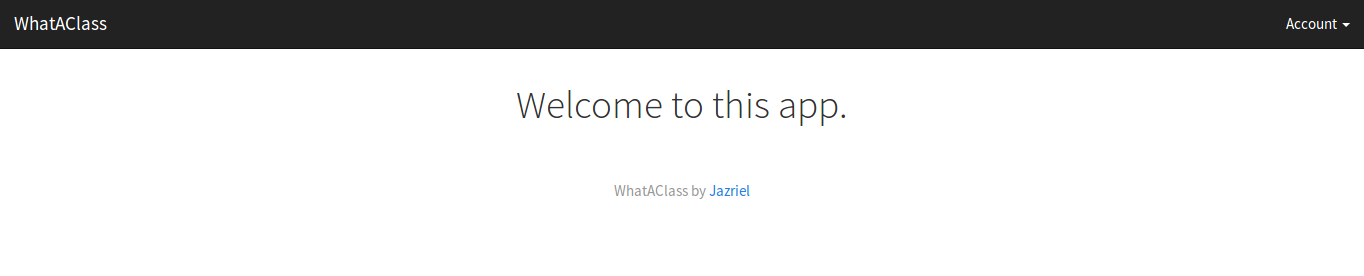
\includegraphics[width=0.8\textwidth]{index.png}
	\caption{Punto de entrada a la aplicación}\label{fig:index.png}
\end{figure}

Para usar la aplicación a partir de ese punto necesita registrarse o iniciar sesión con una de las cuentas alternativas.

\begin{figure}
	\centering
	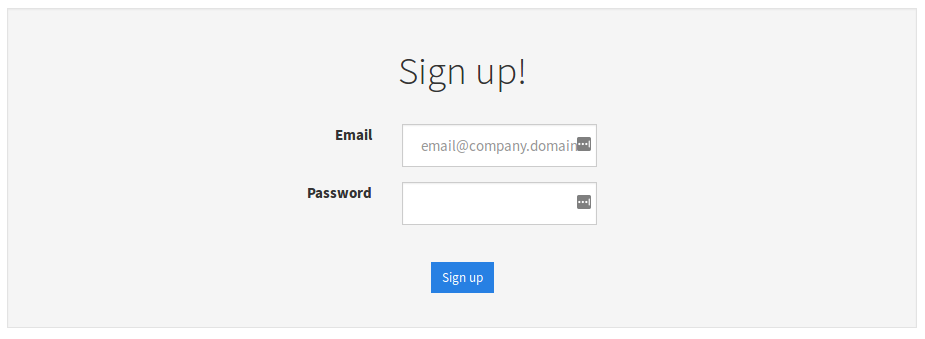
\includegraphics[width=0.8\textwidth]{signup.png}
	\caption{Pantalla de registro de usuario}\label{fig:signup.png}
\end{figure}

Tras registrarse como usuario o tripulante, si esta preparado el correo, se envía un correo electrónico a su dirección personal.

\begin{figure}
	\centering
	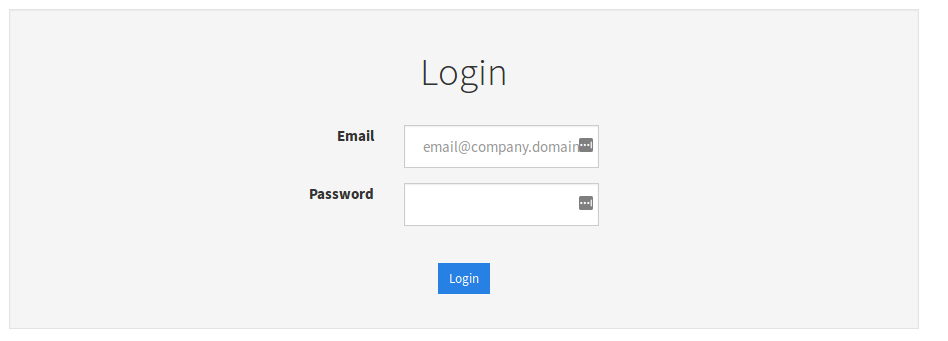
\includegraphics[width=0.8\textwidth]{login.png}
	\caption{Pantalla de inicio de sesión}\label{fig:login.png}
\end{figure}

Una vez se confirma la recepción del correo, se activa la cuenta, permitiendo así usar servicios que antes no estaban disponibles.

\begin{figure}
	\centering
	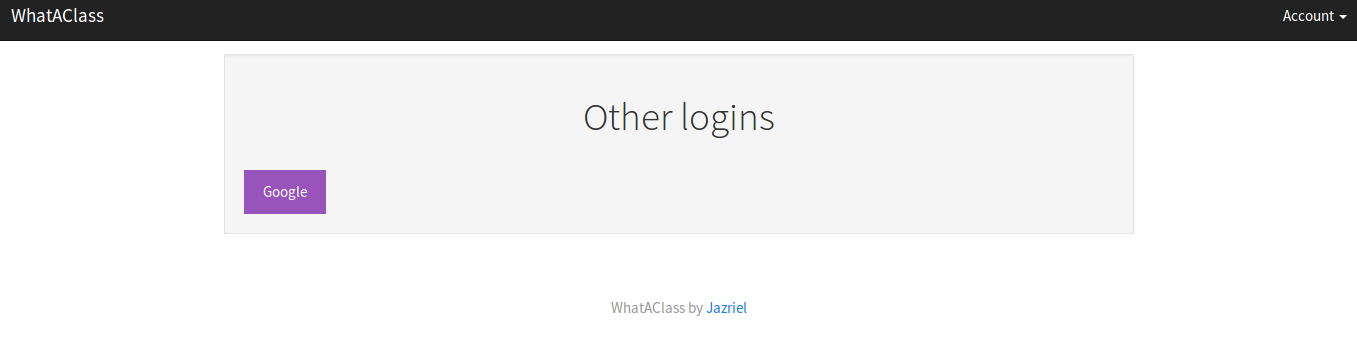
\includegraphics[width=0.8\textwidth]{other_logins.png}
	\caption{Inicios de sesión alternativos}\label{fig:other_logins.png}
\end{figure}


\begin{figure}
	\centering
	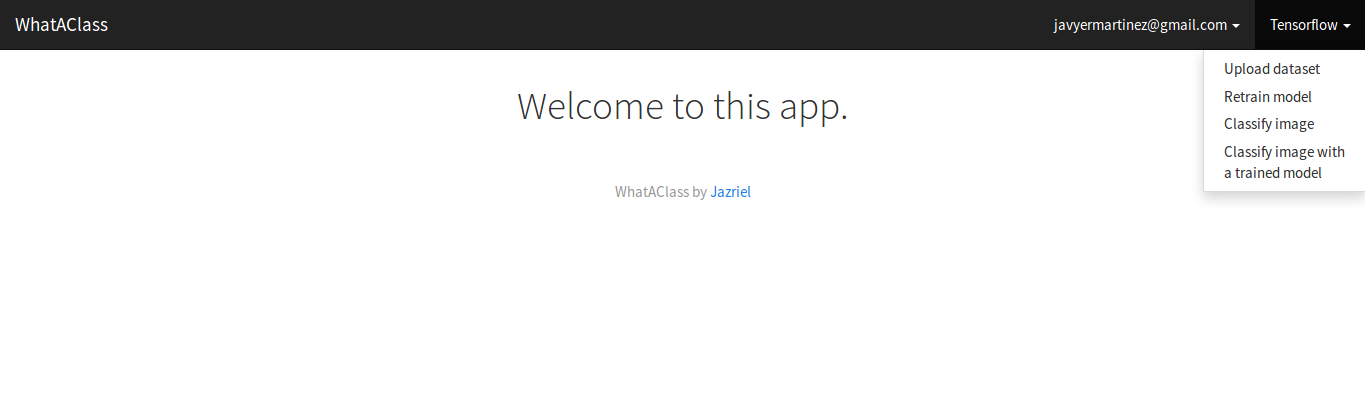
\includegraphics[width=0.8\textwidth]{loggedin.png}
	\caption{Cambio de las zonas accesibles al iniciar sesión}\label{fig:loggedin.png}
\end{figure}


\begin{figure}
	\centering
	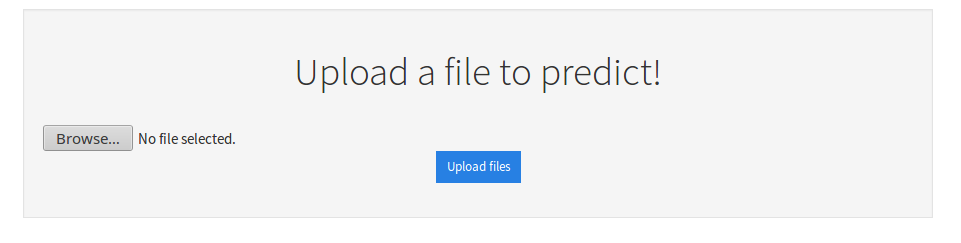
\includegraphics[width=0.8\textwidth]{predict.png}
	\caption{Pantalla de acceso a el servicio de clasificación}\label{fig:predict.png}
\end{figure}






